\section{Datasets and Evaluation}
\label{sec:evaluation}
\subsection{Datasets and Degradation Protocols}
Evaluation of diffusion-based video restoration combines three complementary sources of evidence: reconstruction on paired data, perceptual assessment on real degraded videos, and temporal analysis over continuous sequences. REDS and Vimeo90K provide widely used source material for controlled restoration studies~\cite{reds,vimeo90k}. Synthetic degradation makes the reference target and corruption process explicit, enabling comparisons across degradation strengths and combinations. Its limitation is the difference between the simulated operator and real acquisition. RealBasicVSR's VideoLQ contains real low-quality videos without matched clean references~\cite{realbasicvsr}, supporting the study of practical artifacts and robustness while providing less direct evidence about recovery of the original scene.

Specialized domains introduce additional relationships between data and evaluation. Face restoration depends on identity preservation; underwater enhancement involves uncertainty about scene color; infrared sequences vary with sensor response; and HDR reconstruction depends on the radiometric and display pipeline. Generated video presents a different problem because a unique clean reference may not exist and enhancement can change the generated content itself. Table~\ref{tab:data} summarizes these complementary evaluation settings. Together, they cover aspects of restoration that a single dataset or aggregate score cannot adequately represent.

\begin{table*}[t]
\caption{Data settings for evaluating video restoration and enhancement. Each setting provides a different form of evidence about reconstruction, perceptual quality, or temporal behavior.}
\label{tab:data}\centering\footnotesize
\begin{tabularx}{\textwidth}{@{}p{0.18\textwidth}YYY@{}}\toprule
Data setting & Typical data / examples & Evaluation focus & Main limitation \\\midrule
Paired synthetic & Clean video with simulated degradation; REDS or Vimeo90K-derived protocols~\cite{reds,vimeo90k} & Controlled reconstruction, severity variation, degradation mixtures & Difference between simulation and real acquisition \\
Paired real & Matched captures with aligned references & Real degradation and reference-based fidelity & Misregistration, sensor differences, target uncertainty \\
Unpaired real & In-the-wild low-quality video; VideoLQ~\cite{realbasicvsr} & Practical robustness, preference, visible artifacts & Limited evidence about recovery of the original scene \\
Specialized domain & Face, underwater, thermal, HDR, and event-conditioned sequences & Identity, physical consistency, radiometry, domain shift & Domain-specific acquisition conditions and quality criteria \\
Generated video & Outputs from held-out generators and prompts & Artifact correction, content preservation, motion plausibility & Absence of a unique clean reference \\
Long/streaming video & Continuous shots, cuts, occlusions, changing corruption & Drift, delay, state resets, boundary behavior & Failures obscured by short-clip averages \\\bottomrule
\end{tabularx}
\end{table*}

The degradation protocol is as consequential as the source dataset. Resampling, noise, blur, and compression interact through their order and temporal structure. Changing these choices can alter method rankings even when the clean videos remain unchanged. Generalization also depends on the partitioning unit: adjacent frames from one sequence are highly related, while different captures may share scene content, identities, or acquisition characteristics. Sequence-level partitions and held-out capture or generation pipelines provide stronger evidence of transfer than frame-level splits. Fixed degradation realizations further reduce variation unrelated to the restoration method.

\subsection{Objective Quality Assessment}
\textbf{Reference-based distortion.} PSNR and structural similarity quantify agreement with a clean reference and are particularly informative for reconstruction under controlled, well-aligned conditions. They penalize plausible details that differ from the target, making them sensitive to the fidelity side of the perception--distortion trade-off. Their values also depend on color space, channel selection, border cropping, and alignment. Averaging framewise scores summarizes a sequence compactly, but may conceal brief or spatially localized failures.

\textbf{Perceptual similarity.} LPIPS compares deep image features, while DISTS combines structure- and texture-sensitive components~\cite{lpips,dists}. These measures tolerate some changes that contribute substantially to pixel error but have a smaller perceptual effect. Their use in video is commonly framewise, so temporal instability can remain undetected after averaging. Texture tolerance can also obscure whether generated details remain attached to the correct moving surface. Perceptual image similarity and temporal consistency consequently provide different information about a restored sequence.

\textbf{No-reference video quality.} FAST-VQA and DOVER estimate video quality without a clean target using different sampling and modeling strategies~\cite{fastvqa,dover}. They extend evaluation to real videos for which reference-based scores are unavailable. Their reliability depends on the relationship between the training distribution and the restoration outputs being assessed. Diffusion-based restoration can produce combinations of sharpness, unsupported detail, geometric displacement, and flicker that differ from conventional user-generated-content distortions, creating a potential mismatch between learned predictions and viewer judgments.

\textbf{Temporal measures.} Motion-compensated residuals, such as Eq.~\eqref{eq:warp}, quantify appearance agreement along estimated motion. Their interpretation depends on optical-flow accuracy, occlusion handling, and the amount of motion retained by the restored output. Excessive smoothing or suppressed motion can reduce a residual without improving restoration. Flicker, identity persistence, motion accuracy, and scene-cut behavior are related but distinct temporal properties; reference motion, when available, helps distinguish faithful dynamics from internal smoothness alone.

\textbf{Distributional and generation-oriented measures.} FVD compares feature distributions across sets of videos~\cite{fvd}, whereas VBench decomposes video generation quality into several dimensions, including temporal behavior~\cite{vbench}. These measures offer useful diagnostics for generative outputs. However, distributional plausibility does not establish correspondence between a restored video and its degraded input. A plausible population of outputs can still contain changes to particular objects, identities, or events. Restoration therefore couples these diagnostics with measures of input or reference consistency.

\begin{table*}[t]
\caption{Complementary objective and subjective measures for video restoration. Their sensitivities explain why evaluation combines spatial fidelity, perceptual quality, and temporal behavior.}
\label{tab:metrics}\centering\footnotesize
\begin{tabularx}{\textwidth}{@{}p{0.20\textwidth}YYY@{}}\toprule
Metric family & Main quantity assessed & Main sensitivity / limitation & Complementary evidence \\\midrule
PSNR / SSIM & Agreement with a clean reference & Misalignment; perceptually minor changes; frame averaging & Perceptual similarity and temporal diagnostics \\
LPIPS / DISTS~\cite{lpips,dists} & Similarity of perceptual image features & Framewise assessment; tolerance of texture changes & Motion-compensated and structural consistency \\
FAST-VQA / DOVER~\cite{fastvqa,dover} & Learned no-reference video quality & Domain shift; content bias; preference for sharpness & Human assessment of restored outputs \\
Warping / temporal features & Appearance agreement along motion & Flow errors; occlusions; excessive smoothing & Reference motion and disocclusion analysis \\
FVD / VBench~\cite{fvd,vbench} & Distributional or dimensional plausibility & Limited sensitivity to conditioning fidelity; sample dependence & Input consistency and task-specific assessment \\
Human judgments & Perceived quality under a specified viewing task & Display conditions; instructions; observer variation & Separate quality questions and statistical uncertainty \\\bottomrule
\end{tabularx}
\end{table*}

\subsection{Subjective Assessment of Diffusion-Based VSR}
Herb et al.~\cite{metric} examine the reliability of objective predictors in \emph{How Accurate are Video Quality Models for Diffusion-Based Video Super-Resolution?} The study uses six source clips of 8--10 seconds at UHD resolution and 60 frames per second. Inputs are downscaled to 360p or 720p under AV1, DCVC-RT, and uncompressed conditions. Six upscalers produce the material for an evaluation comprising 222 test sequences, including original UHD references. The subjective experiment recruits 32 observers and retains 28 after screening. It uses five-point absolute category ratings on a 43-inch UHD display at a viewing distance of 1.5 picture heights.

The study distinguishes within-source correlations from overall correlations. The former measure how well a predictor ranks different versions of the same source and are aggregated using Fisher transformation; the latter combine the evaluated material across sources. Figure~\ref{fig:metriccorrelations} visualizes all 30 pairs of SRCC values reported in Table I of the study. LPIPS (Alex), for example, changes from 0.881 within sources to 0.636 overall, while DISTS changes from 0.850 to 0.712. Among no-reference predictors, FasterVQA changes from 0.683 to 0.538 and MDTVSFA from 0.529 to 0.263. These differences show that ranking restorations within a scene and comparing quality across different content are distinct evaluation problems.

\begin{figure*}[t]
\centering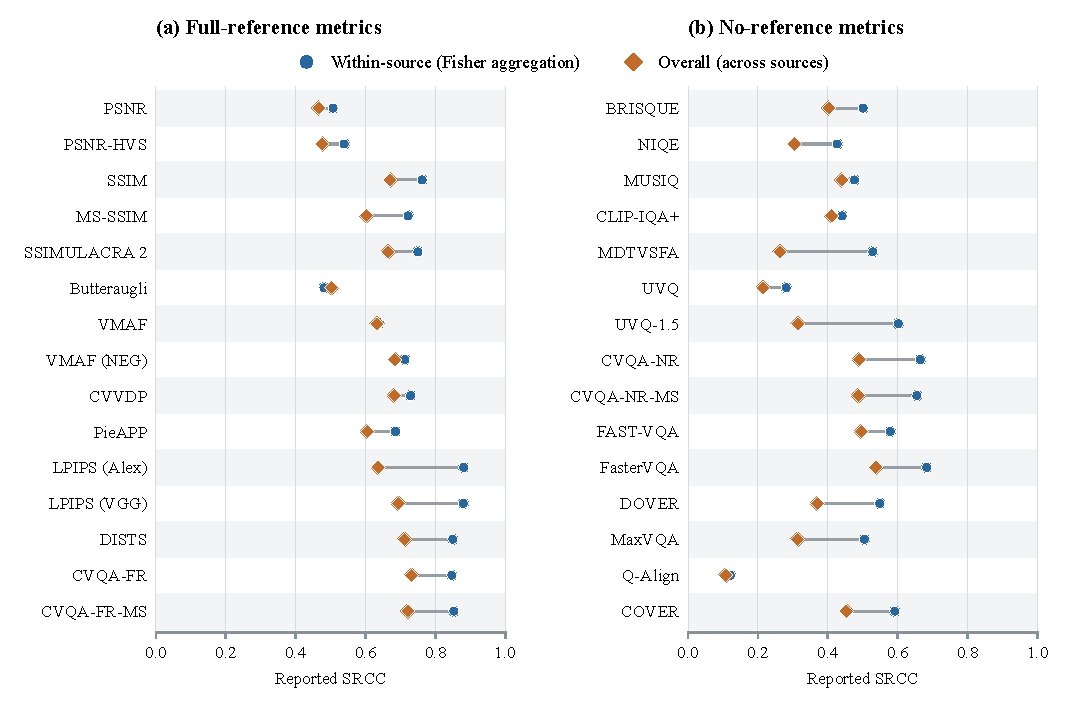
\includegraphics[width=\textwidth]{figures/benchmark.pdf}
\caption{Reported agreement between objective predictions and subjective scores for diffusion-based VSR. All 30 SRCC pairs are redrawn from Herb et al.~\cite{metric}, Table I, in the original table order. Circles show within-source correlations aggregated by Fisher transformation; diamonds show overall correlations across sources. Lines connect the two reported values for a metric, rather than uncertainty intervals. The study retains 28 observers and uses six source clips; the reported values and sign conventions are preserved. Table I supplies no SRCC confidence intervals. These results characterize the study's tested content and configurations.}
\label{fig:metriccorrelations}
\end{figure*}

Neural full-reference predictors provide useful ranking information in this experiment, while no-reference predictors can overrate some oversharpened outputs and pixel metrics are sensitive to small spatial misalignments. These findings support combining objective scores with subjective assessment, particularly when generative detail changes the appearance of a scene. The observed ranking remains specific to the tested content, degradations, methods, and viewing conditions; it does not establish a universal ordering of quality metrics across restoration domains.

Model configuration also influences the interpretation of the study. To fit an A100 with 40 GB memory, the authors adjust temporal batches, overlap, and spatial processing where necessary. These choices can affect temporal consistency and runtime as well as feasibility. The reported timings therefore characterize the evaluated configurations and cannot be transferred directly to methods running with different processing windows or hardware. This illustrates the close relationship between visual quality, implementation choices, and resource constraints in diffusion-based VSR.

\subsection{Fair Comparison Across Backbones}
Restoration methods increasingly draw on different pretrained image and video models, whose training data, capacity, temporal representations, and generative quality vary substantially. Comparing their final outputs reveals useful system-level progress, but does not by itself isolate the contribution of a restoration mechanism. A shared model family also does not guarantee matched pretraining or initialization. These differences motivate separating controlled comparison from comparison of complete systems.

\textbf{Controlled comparison.} This track examines conditioning strategies, temporal coupling, objectives, or samplers under matched resources. A common prior checkpoint, training-data access, degradation protocol, resolution, temporal context, sampling budget, and side information reduce confounding factors. Total and trainable parameter counts account for auxiliary components such as adapters, decoders, and flow networks. Some mechanisms are closely tied to a particular backbone and cannot be transferred without changing their operation. In those cases, matched ablations within the original system provide more interpretable evidence than a nominally shared backbone that alters the method itself.

\textbf{Complete-system comparison.} This track retains each system's intended backbone and training recipe while using common test clips and evaluation conditions. It measures the quality--cost operating points available in practice. Model capacity, training data, external references, temporal context, and the computational cost of auxiliary components remain relevant explanatory variables. Such comparisons reveal the benefits of integrating stronger priors and restoration designs, although the resulting differences cannot be attributed exclusively to one architectural or algorithmic component.

The tracks address complementary questions. Controlled comparison supports analysis of restoration mechanisms; complete-system comparison captures advances in available models and their practical deployment. Together, they avoid interpreting all gains from stronger pretraining as gains from a new mechanism, while allowing the survey of system progress to include current backbones.

\subsection{Evaluation Practice}
Reproducibility in diffusion-based video restoration depends on both the model and the inference procedure. Checkpoint versions, training-data access, auxiliary models, and available conditioning determine the information used for restoration. Sampling steps, guidance, stochastic seeds, temporal windows, spatial tiles, and overlap determine how that information is processed. For long or streaming videos, future-frame access, cache behavior, and state resets further affect latency and temporal continuity. Reporting these settings alongside metric preprocessing, hardware, precision, and timing boundaries makes comparisons interpretable across implementations.

Human assessment separates questions that an overall preference may combine: viewing quality, preservation of source content, and temporal artifacts. Whether observers see the degraded input, a clean reference, both, or neither changes the judgment being elicited. Anonymized methods, randomized presentation, and documented playback and display conditions reduce avoidable variation. Subjective assessment is especially valuable for real degraded or generated videos, where a reliable reference may be unavailable, and for generative artifacts that existing quality models represent poorly.

Statistical analysis likewise reflects the structure of video data. Neighboring frames are correlated, making sequence- or content-level resampling more informative than treating every frame as an independent observation. Observer variation contributes additional uncertainty in subjective experiments. Aggregate results gain interpretability from analyses of large motion, occlusion, fine text, scene cuts, and severe degradation. For stochastic restorers, common seed sets and variation across repeated outputs distinguish reliable improvements from favorable individual samples.

Finally, quality models require validation beyond the restoration systems and content used for their calibration. Held-out model families and degradation processes test whether a predictor remains useful when the characteristic artifacts change. At the method level, reporting fidelity, perceptual quality, temporal stability, and cost separately exposes operating points and trade-offs that a single weighted score may conceal. This multidimensional view connects evaluation directly to the central objectives of diffusion-based video restoration.
